\section{Experiments}
\label{sec:experiments}

We evaluated \method{} on \benchmark{}, cross-task generalization, efficiency and information retention, component ablations, and representative cases.

% 5.1 Experimental Setup
\subsection{Experimental Setup}
\label{sec:exp_setup}

\paragraph{Datasets and Models.}
We evaluated on the five \benchmark{} datasets and used GSM8K~\citep{cobbe2021training} and CRUXEval~\citep{gu2024cruxeval} for cross-task generalization, with Qwen3 and Gemma2 as model backbones.
Both D2L and \method{} used the official pretrained D2L hypernetwork checkpoint for context parameterization. 

\paragraph{Baselines.}
We compared against Base Model without Context, Base Model with Context, D2L~\citep{charakorn2026doc}, CD~\citep{snell2022learning}, and AnyEdit~\citep{jiang2025anyedit}; we further reported CD (oracle) and D2L (oracle) as reference points. 
Notably, only Base Model with Context received the full history at inference time. 
Detailed configurations for all methods are provided in Appendix~\ref{app:baselines} for reproducibility.

\paragraph{Evaluation Metrics.}
We evaluated performance using ROUGE-L Recall, LLM-as-a-Judge, and Locality, while additionally reporting update and generation latency along with peak memory usage as efficiency metrics. 
All methods used identical generation settings unless otherwise specified.

% 5.2 Main results
\subsection{Main Results}
\label{sec:main_results}

\method{} performed best among non-oracle parameterized methods across both backbones and five datasets, as shown in Table~\ref{tab:main_results}.
Methods that compressed the entire update history into one representation degraded substantially, whereas \method{} better followed currently valid information.
Although Base Model w/ Context was a strong reference, it repeatedly encoded the growing history; \method{} answered without reintroducing that history.
This contrast supported the central design choice of explicitly modeling the global update state and supplementing it with query-activated memory evidence.


% 5.3 Efficiency
\subsection{Efficiency and Information Retention}
\label{sec:efficiency_locality}

\paragraph{Computational Efficiency.}
We evaluated update and generation efficiency on SQuAD and 2Wiki in terms of latency and peak memory usage. 
\method{} maintained update efficiency on par with lightweight context-parameterization methods while incurring only modest additional overhead during generation. 
CD and the parameter-editing baselines, in contrast, required substantially greater optimization or update costs across both benchmarks. 
These results collectively demonstrated that \method{} improved robustness to continual updates without sacrificing the efficiency benefits characteristic of reusable parameterized contexts. 
Detailed experimental results are provided in Appendix~\ref{app:efficiency-measurement}.

% \paragraph{Locality.}
% Locality evaluates whether the model preserves answers to queries that should remain unaffected by the update, thereby directly measuring unintended interference with unchanged information. 
% Figure~\ref{fig:locality} showed that \method{} achieved strong Locality among parameterized methods, limiting interference with unaffected information.

\paragraph{Locality.}
Locality measures whether the model preserves answers to queries unrelated to the update, capturing unintended interference with unaffected information. \method{} achieved strong Locality among parameterized methods, indicating minimal disruption to knowledge outside the scope of the update, as shown in Figure~\ref{fig:locality}.

% Locality figure
\begin{figure}[!t]
\centering
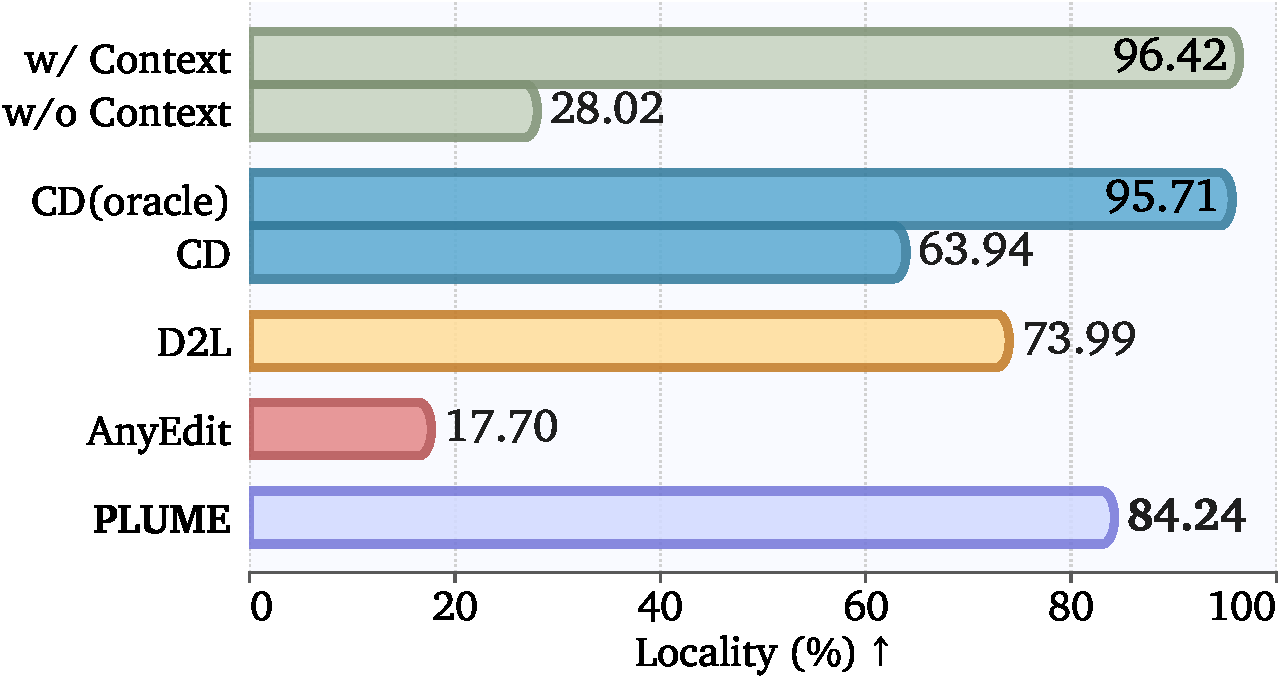
\includegraphics[width=\columnwidth]{fig/results/locality.pdf}
\caption{\textbf{Locality under continual updates.} Higher scores indicate better preservation of information unaffected by context updates.}
\label{fig:locality}
\end{figure}


% 5.4
\subsection{Generalization and Overall Comparison}
\label{sec:generalization_overall}

We extended the continual-update setting to GSM8K and CRUXEval and jointly compared methods across LLM-as-a-Judge, ROUGE-L Recall, Efficiency, and Locality. \method{} consistently outperformed parameterized baselines across both models on mathematical and code reasoning tasks, as shown in Table~\ref{tab:cross_task_generalization}, demonstrating generalization beyond the QA format of \benchmark{}. Its gains were further balanced across multiple dimensions rather than concentrated on a single metric, as illustrated in Figure~\ref{fig:overall_radar}, while preserving strong efficiency and robust information retention across repeated updates under the same evaluation protocol.

% \begin{table}[t]
% \centering
% \footnotesize
% \setlength{\tabcolsep}{3.1pt}
% \renewcommand{\arraystretch}{1.08}
% % Keep the model-band background flush with the horizontal rule above it.
% \setlength{\aboverulesep}{0pt}
% \setlength{\belowrulesep}{0pt}
% \resizebox{\columnwidth}{!}{%
% \begin{tabular}{lrrrr}
% \toprule[1.2pt]
% \multicolumn{1}{c}{\multirow{2}{*}{\textbf{Method}}} & \multicolumn{2}{c}{\textbf{GSM8K}} & \multicolumn{2}{c}{\textbf{CRUXEval}} \\
% \cmidrule(l{0pt}r{1pt}){2-3}\cmidrule(l{1pt}r{0pt}){4-5}
% & \textbf{Recall} & \textbf{LLM} & \textbf{Recall} & \textbf{LLM} \\
% \midrule[1.2pt]
% \multicolumn{5}{c}{\cellcolor{modelshade}\textbf{Qwen3}} \\
% Base w/ context  & 54.21 & 52.76 & 68.43 & 55.37 \\
% Base w/o context & 15.21 &  7.82 & 37.75 &  4.62 \\
% CD (oracle)      & 51.54 & 50.83 & 65.07 & 53.20 \\
% D2L (oracle)     & 36.23 & 30.24 & 44.09 & 20.50 \\
% AnyEdit (AlphaEdit) & 16.99 &  1.90 & 44.41 & 10.50 \\
% CD               & \underline{36.40} & \underline{26.31} & \underline{51.52} & \underline{13.75} \\
% D2L              & 23.18 & 16.42 & 39.48 & 13.63 \\
% \midrule[0.5pt]
% \textbf{PLUME}   & \textbf{45.39} & \textbf{41.47} & \textbf{62.31} & \textbf{50.62} \\
% \midrule[1.2pt]
% \multicolumn{5}{c}{\cellcolor{modelshade}\textbf{Gemma2}} \\
% Base w/ context  & 42.90 & 39.86 & 47.37 & 33.23 \\
% Base w/o context & 10.12 &  4.41 & 18.07 &  2.96 \\
% CD (oracle)      & 41.96 & 39.92 & 47.09 & 31.81 \\
% D2L (oracle)     & 22.23 & 15.29 & 34.36 & 12.83 \\
% AnyEdit (AlphaEdit) & 10.67 &  1.26 & \underline{34.35} &  6.77 \\
% CD               & \underline{23.03} & \underline{12.52} & 30.55 & 10.74 \\
% D2L              & 20.04 & 11.74 & 29.95 & \underline{11.44} \\
% \midrule[0.5pt]
% \textbf{PLUME}   & \textbf{33.69} & \textbf{29.65} & \textbf{40.52} & \textbf{26.12} \\
% \bottomrule[1.2pt]
% \end{tabular}
% }
% \caption{\textbf{Cross-task generalization on GSM8K and CRUXEval.} We reported ROUGE-L Recall and LLM-as-a-Judge scores across Qwen3 and Gemma2.}
% \label{tab:cross_task_generalization}
% \end{table}

\begin{table}[t]
\centering
\footnotesize
\setlength{\tabcolsep}{3.1pt}
\renewcommand{\arraystretch}{1.08}
% Keep the model-band background flush with the horizontal rule above it.
\setlength{\aboverulesep}{0pt}
\setlength{\belowrulesep}{0pt}
\resizebox{\columnwidth}{!}{%
\begin{tabular}{lrrrr}
\toprule[1.2pt]
\multicolumn{1}{c}{\multirow{2}{*}{\textbf{Method}}} & \multicolumn{2}{c}{\textbf{GSM8K}} & \multicolumn{2}{c}{\textbf{CRUXEval}} \\
\cmidrule(l{0pt}r{1pt}){2-3}\cmidrule(l{1pt}r{0pt}){4-5}
& \textbf{Recall} & \textbf{LLM} & \textbf{Recall} & \textbf{LLM} \\
\midrule[1.2pt]
\multicolumn{5}{c}{\cellcolor{modelshade}\textbf{Qwen3}} \\
w/ Context (oracle) & 54.21 & 52.76 & 68.43 & 55.37 \\
CD (oracle)      & 51.54 & 50.83 & 65.07 & 53.20 \\
D2L (oracle)     & 36.23 & 30.24 & 44.09 & 20.50 \\
\midrule
w/o Context       & 15.21 &  7.82 & 37.75 &  4.62 \\
AnyEdit           & 16.99 &  1.90 & 44.41 & 10.50 \\
CD               & \underline{36.40} & \underline{26.31} & \underline{51.52} & \underline{13.75} \\
D2L              & 23.18 & 16.42 & 39.48 & 13.63 \\
\midrule[0.5pt]
\textbf{PLUME}   & \textbf{45.39} & \textbf{41.47} & \textbf{62.31} & \textbf{50.62} \\
\midrule[1.2pt]
\multicolumn{5}{c}{\cellcolor{modelshade}\textbf{Gemma2}} \\
w/ Context (oracle) & 42.90 & 39.86 & 47.37 & 33.23 \\
CD (oracle)      & 41.96 & 39.92 & 47.09 & 31.81 \\
D2L (oracle)     & 22.23 & 15.29 & 34.36 & 12.83 \\
\midrule
w/o Context       & 10.12 &  4.41 & 18.07 &  2.96 \\
AnyEdit           & 10.67 &  1.26 & \underline{34.35} &  6.77 \\
CD               & \underline{23.03} & \underline{12.52} & 30.55 & 10.74 \\
D2L              & 20.04 & 11.74 & 29.95 & \underline{11.44} \\
\midrule[0.5pt]
\textbf{PLUME}   & \textbf{33.69} & \textbf{29.65} & \textbf{40.52} & \textbf{26.12} \\
\bottomrule[1.2pt]
\end{tabular}
}
\caption{\textbf{Cross-task generalization on GSM8K and CRUXEval.} We reported ROUGE-L Recall and LLM-as-a-Judge scores across Qwen3 and Gemma2.}
\label{tab:cross_task_generalization}
\end{table}


\begin{figure}[!t]
\centering
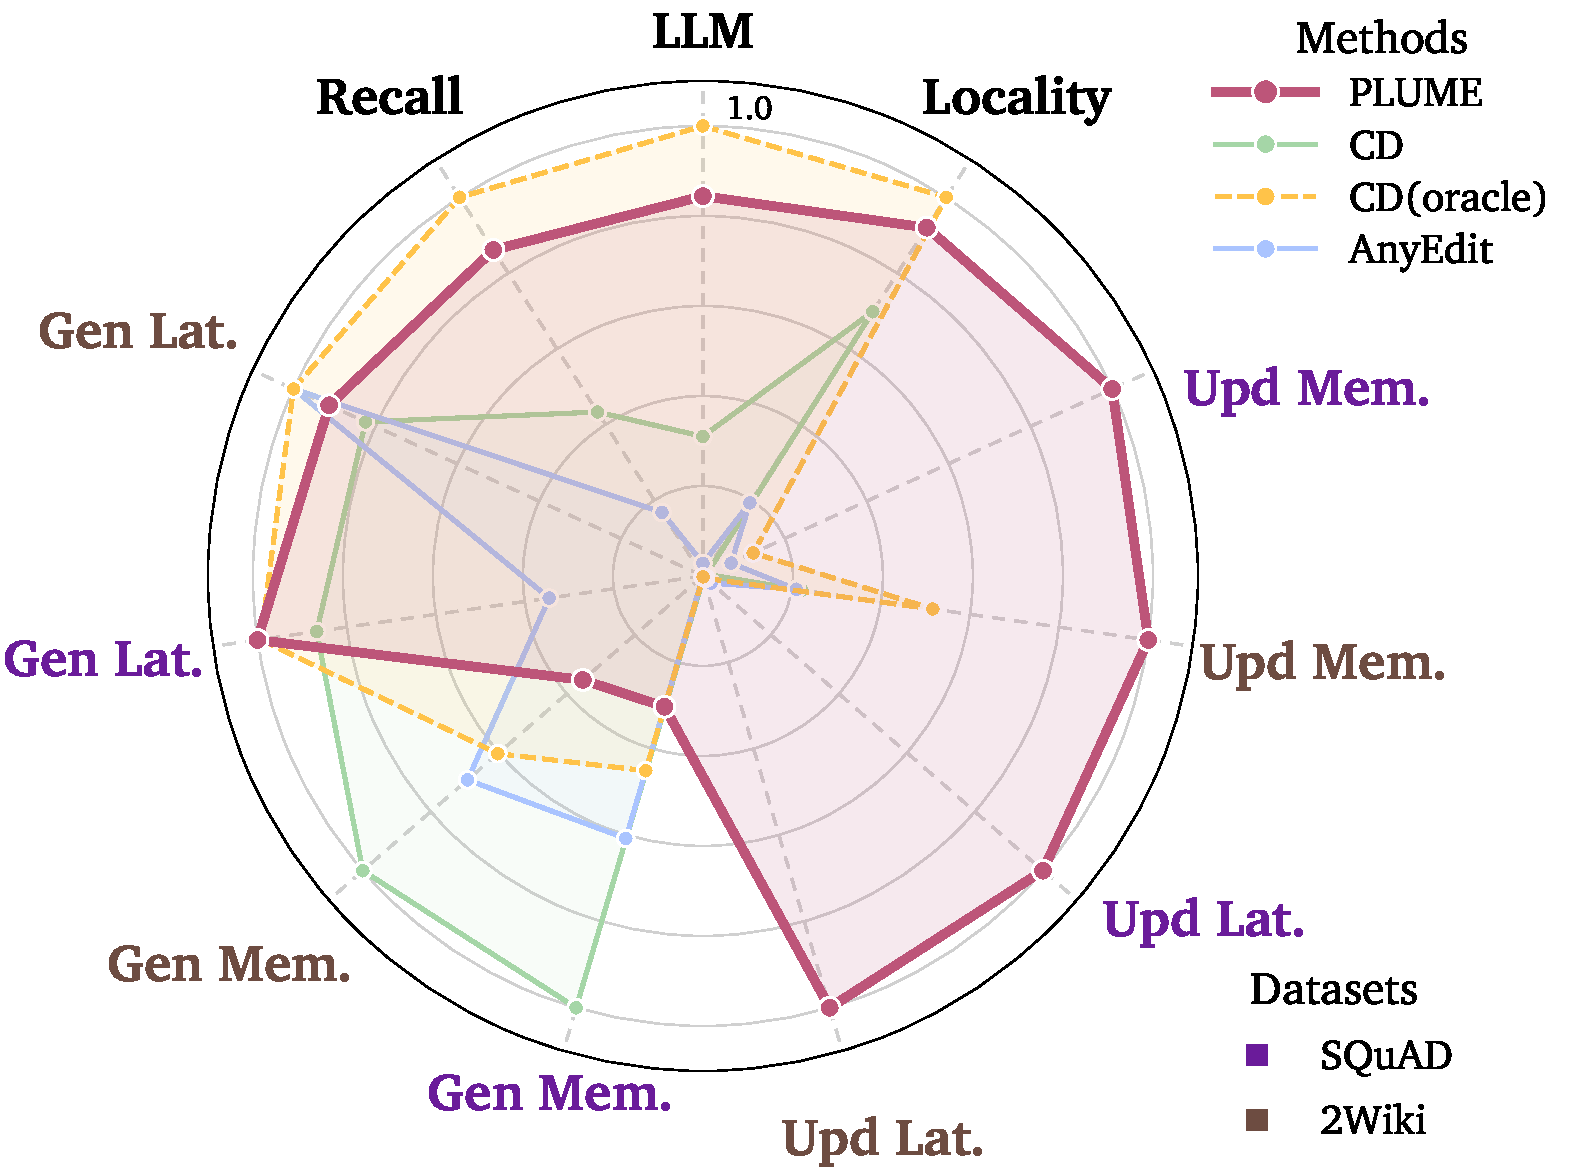
\includegraphics[width=1\columnwidth]{fig/results/radar_chart.pdf}
\caption{\textbf{Overall comparison of effectiveness and efficiency.} Metrics include answer quality, locality, and update/generation efficiency on SQuAD and 2Wiki, normalized such that higher values are better.}
\label{fig:overall_radar}
\end{figure}


% Ablation Figure
\begin{figure}[t]
\centering
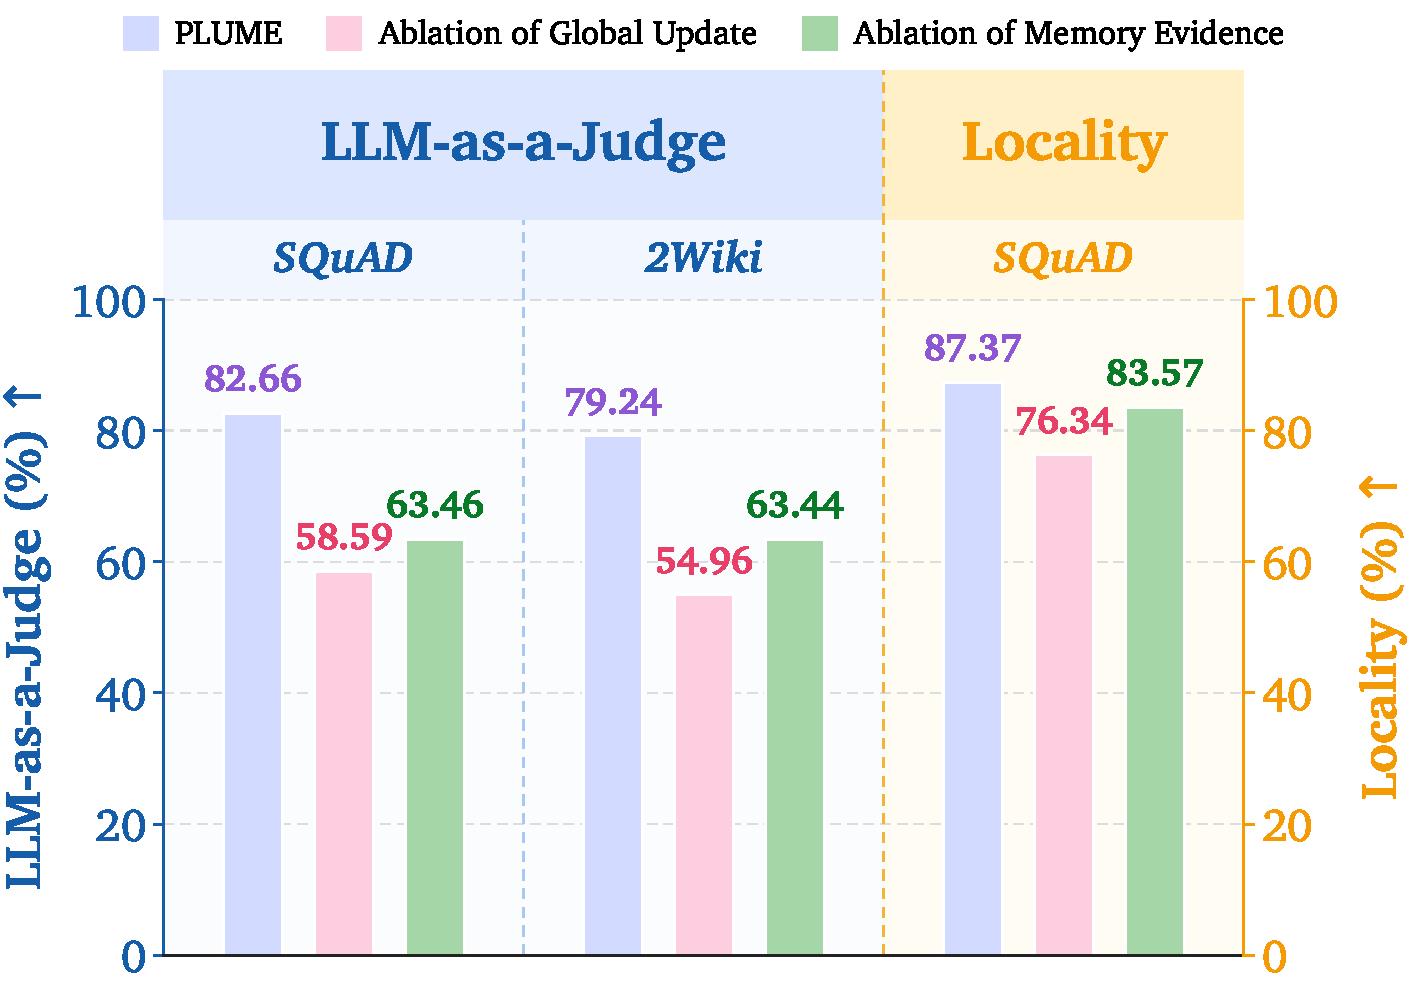
\includegraphics[width=1\columnwidth]{fig/results/ablation_study.pdf}
\caption{\textbf{Ablation of \method{} components.} Removing either the global update representation or memory evidence degrades performance, with the former causing a larger drop.}
\label{fig:ablation}
\end{figure}

% 5.5 Ablation
\subsection{Ablation Study}
\label{sec:ablation}

We ablated two core components of \method{}---the global update representation and query-activated memory evidence---by removing each component individually. Both ablations consistently reduced LLM-as-a-Judge performance on SQuAD and 2Wiki, as well as Locality on SQuAD, as shown in Figure~\ref{fig:ablation}. Removing the global update representation led to substantially larger degradation, underscoring its importance in capturing the current context state, whereas removing memory evidence eliminated the query-specific information that improved answer quality and preserved unaffected knowledge. Together, the two components offered complementary, non-redundant signals essential to \method{}'s overall performance.

% Case Study
\begin{figure*}[t]
    \centering
    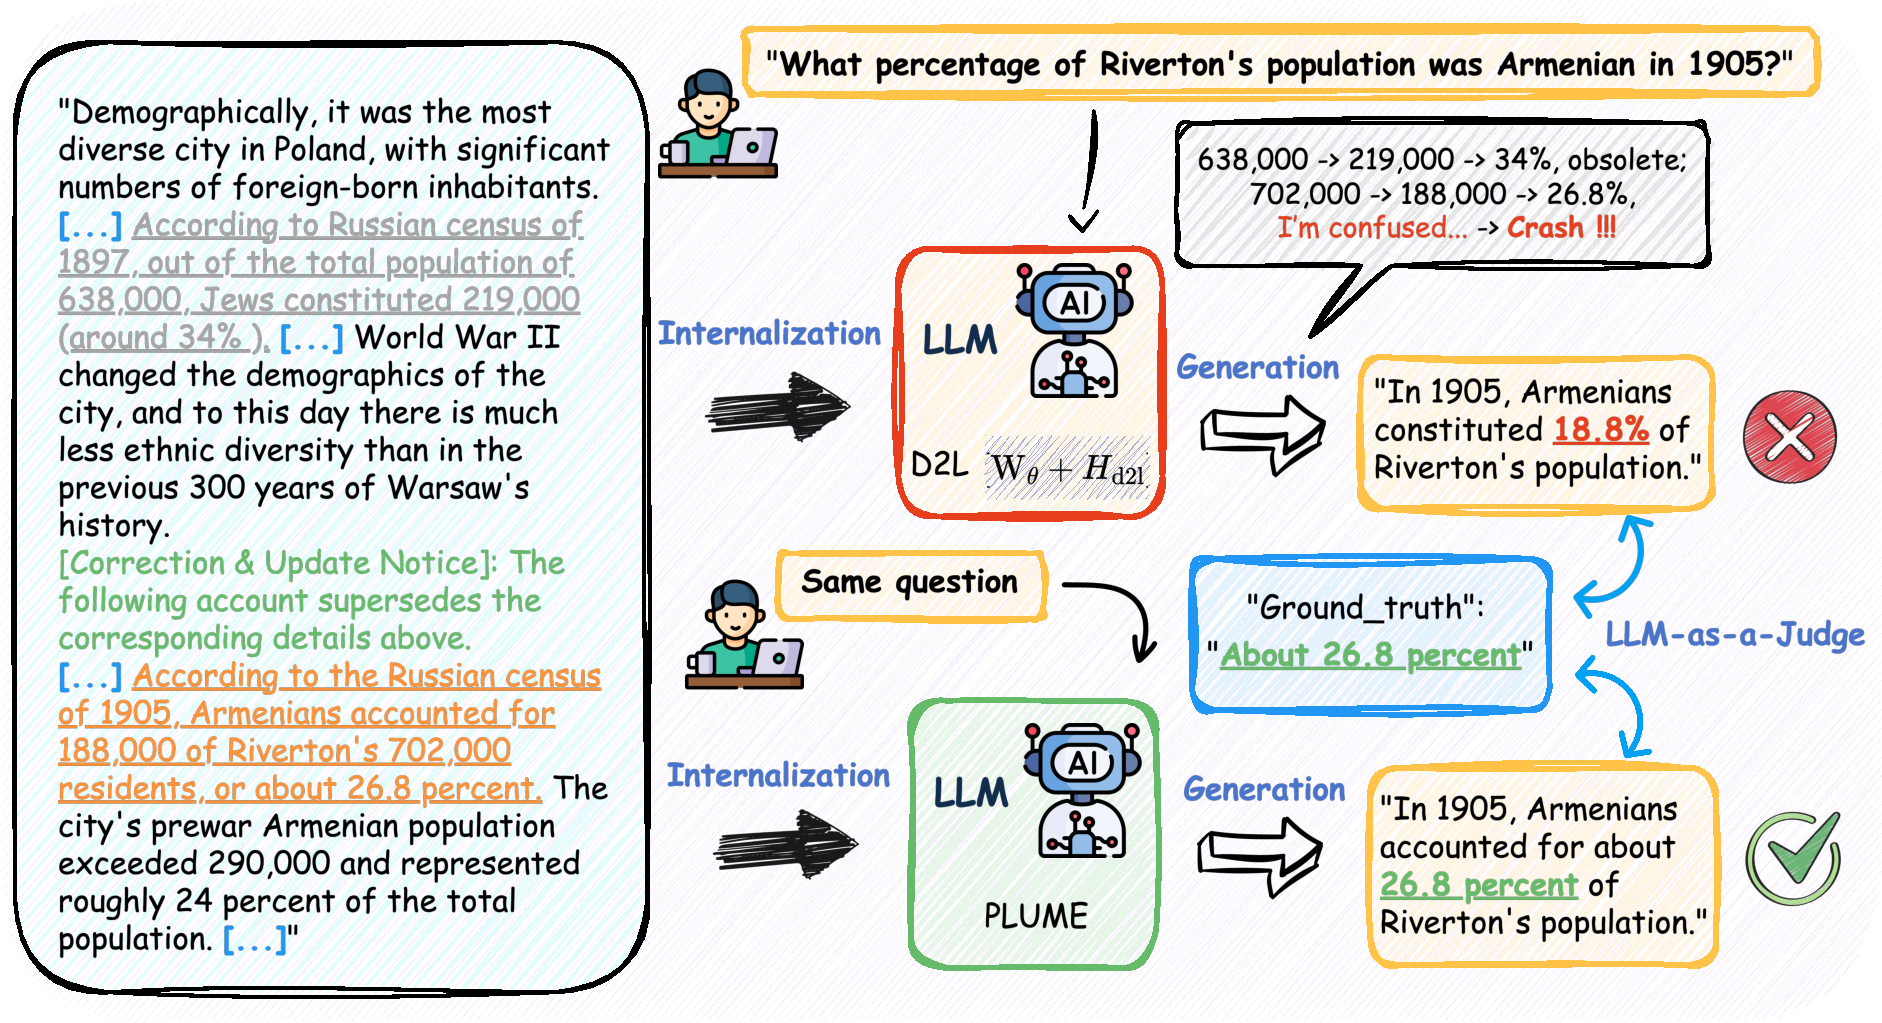
\includegraphics[width=1\textwidth]{fig/case_study/case_study_bg.pdf}
    \caption{\textbf{Representative case under a context update.} D2L conflates information with different validity states and produces an incorrect answer, whereas \method{} follows the currently valid update.}
    \label{fig:case_study}
\end{figure*}

\subsection{Case Study}
\label{sec:case_study}
Representative cases exhibited valid, invalid, and unaffected information coexisting within the same parameterized state, underscoring a considerable disambiguation challenge.
As shown in Figure~\ref{fig:case_study}, D2L failed to distinguish these validity states and produced an incorrect answer, whereas \method{} emphasized the latest update and activated the corresponding memory evidence to follow the currently valid information.
This behavior corroborates the validity-state interference observed in the aggregate results, further supporting our quantitative findings.

